\chapter{Training the Final Model}\label{ch:training}

\section{Introduction}\label{sec:train-first}
\epigraph{We should forget about small efficiencies, say about 97\% of the time: premature
optimization is the root of all evil.}{Donald Knuth, \emph{Structured Programming with go to
Statements} \citeyearpar{knuth1974}}

Our first Mask2Former, exp046, was trained on a Kaggle TPU. It shrank every photograph from 2048 to
1024 pixels, used the smaller Swin-T backbone and our own re-implementation of the Hungarian loss, and
ran with a batch size of 1 in 16-bit arithmetic with activation checkpointing. The session limit
stopped it after 2,309 steps, and it scored 0.300 on validation. A continuation (exp058) trained for
about 1,600 more steps, bringing the total to about four epochs of the fifty that had been planned,
and its score fell to 0.247. Submitted as a probe, it appeared on the leaderboard as 0.20. Fused with
the eight-view predictions of the YOLO models (exp048), it also lowered their score, from 0.4571 to
0.4472.

It would have been easy to conclude from this that Mask2Former does not suit filaments. Our
pre-registration (Section~\ref{sec:val-oracles}) explicitly rejected that conclusion, recording that
the architecture had not yet been tested. The model had been stopped a tenth of the way through its
schedule, it had seen the photographs at half their resolution, and its loss was new code that had
never been checked against a reference implementation. None of these results measures the
architecture itself.

This chapter describes the run that did test it, and each of its design choices answers one of the
faults of the first attempt. Section~\ref{sec:train-resolution} measures the cost of resolution and
explains why we never shrink the photograph. Section~\ref{sec:train-sampling} describes how the
training samples are drawn, and Section~\ref{sec:train-optim} the optimiser and its schedule.
Sections~\ref{sec:train-memory}--\ref{sec:train-accumulation} cover memory, speed and a subtle
problem with gradient accumulation, and Section~\ref{sec:train-run} describes the training run
itself.

\section{Resolution: what a mask grid can represent}\label{sec:train-resolution}
Mask2Former predicts masks at a quarter of the size of its input. Since exp046 fed it images of 1024
pixels, its masks lay on a grid of $256\times256$ cells, with one cell for every $8\times8$ native
pixels. Before training again, we measured what this costs (exp136). We took every annotated mask,
averaged it down onto a coarse grid, enlarged it back bilinearly, and thresholded it at one half. The
result is the best that a \emph{perfect} mask head on that grid could produce:
\begin{center}\small
\begin{tabular}{@{}lccc@{}}
\toprule
cell size (native pixels) & mean IoU & thin filaments ($\le3$ px) & IoU above 0.5 \\
\midrule
2 (a 1024 grid) & 0.976 & 0.971 & 100\% \\
\textbf{4 (a 512 grid)} & \textbf{0.914} & \textbf{0.896} & \textbf{99.9\%} \\
8 (a 256 grid) & 0.771 & 0.713 & 95.8\% \\
\bottomrule
\end{tabular}
\end{center}
On a grid with cells of 8 pixels, even a perfect model loses almost a quarter of the IoU on every
filament, and more on thin ones. With cells of 4 pixels, the loss is less than a tenth.
Figure~\ref{fig:train-grid} shows why: a body four pixels wide can be traced by cells four pixels wide,
but not by cells eight pixels wide.

\begin{figure}[t]
\centering
\begin{tikzpicture}
  % (a) 4-pixel cells
  \begin{scope}
    \foreach \cx/\cy in {0/1, 1/1, 2/2, 3/2, 4/3, 5/3, 6/4, 7/4}
      \fill[vizblue!35] (\cx*0.4,\cy*0.4) rectangle ++(0.4,0.4);
    \begin{scope}
      \clip (0,0) rectangle (3.2,2.0);
      \draw[vizorange, line width=0.4cm, opacity=0.55] (-0.2,0.3) -- (3.4,2.1);
    \end{scope}
    \draw[gridline!70!black, line width=0.3pt, step=0.4] (0,0) grid (3.2,2.0);
    \draw[inkmuted, line width=0.6pt] (0,0) rectangle (3.2,2.0);
    \node[note] at (1.6,-0.35) {(a) cells of 4 native pixels};
  \end{scope}
  % (b) 8-pixel cells
  \begin{scope}[xshift=4.6cm]
    \foreach \cx/\cy in {0/0, 1/1, 2/1, 3/2}
      \fill[vizblue!35] (\cx*0.8,\cy*0.8) rectangle ++(0.8,0.8);
    \begin{scope}
      \clip (0,0) rectangle (3.2,2.4);
      \draw[vizorange, line width=0.4cm, opacity=0.55] (-0.2,0.3) -- (3.4,2.1);
    \end{scope}
    \draw[gridline!70!black, line width=0.3pt, step=0.8] (0,0) grid (3.2,2.4);
    \draw[inkmuted, line width=0.6pt] (0,0) rectangle (3.2,2.4);
    \node[note] at (1.6,-0.35) {(b) cells of 8 native pixels};
  \end{scope}
  \fill[vizorange, opacity=0.55] (8.7,1.6) rectangle (9.1,1.8);
  \node[note, anchor=west] at (9.2,1.7) {filament, 4 px wide};
  \fill[vizblue!35] (8.7,1.1) rectangle (9.1,1.3);
  \node[note, anchor=west] at (9.2,1.2) {cells more than\\ half covered};
\end{tikzpicture}
\caption{A filament four pixels wide on two mask grids. With cells of 4 pixels (a), the cells that are
more than half covered trace the body closely. With cells of 8 pixels (b), the best binary trace is a
coarse staircase. The measured ceilings in the table use a smoother encoding than this binary one, but
the ordering is the same. \drawnin{book/chapters/ch12\_training.tex}}
\label{fig:train-grid}
\end{figure}

A second measurement (exp138) put these numbers in context. Scoring one annotator's masks against
another's gave a mean IoU of 0.576, with 74\% of the filaments that both annotators drew above an IoU
of 0.5. Encoding the first annotator's masks on a grid with cells of 4 pixels changed this agreement
by only 0.013. Below cells of 4 pixels, then, any gain in precision is swamped by the differences in
how people draw. Our notes first called this a ``bound'' on the quality of the boundaries, and later
corrected themselves: it measures the agreement between people, and it does not limit what a model
can score against any one of them (Section~\ref{sec:metric-agreement}).

The decision followed directly: \emph{we never shrink the photograph}. Every pixel the model sees is
a native pixel, so its masks come out on the grid with cells of 4 pixels. Two further details keep the
supervision at least that fine. The annotations are rasterised with \texttt{pycocotools} at the native
resolution, using the scorer's own convention (Section~\ref{sec:masks-raster}), and the loss reads
them at fractional point coordinates (Section~\ref{sec:tr-loss}), so the targets are never quantised
to the output grid.

\section{Crops and whole frames}\label{sec:train-sampling}
A batch of eight native $2048\times2048$ frames does not fit on any single GPU that we could rent at a
sensible price, and most of a frame is empty disk anyway. Training therefore uses \keyterm{crops}:
windows of $1024\times1024$ pixels centred on a randomly chosen annotated filament, with the centre
moved at random by up to 35\% of the crop, so that filaments do not always sit in the middle. Since 99\%
of the filaments in the training set are shorter than 516 pixels, a crop almost always contains its
anchor filament whole, and it usually contains several of its neighbours too.

Crops alone, however, would have caused a subtle failure. Section~\ref{sec:tr-positions} noted that the
sine positional embeddings of Equation~\eqref{eq:tr-sine} are normalised by the size of the input. A
model that had only ever seen inputs of 1024 pixels would meet, at test time on a frame of 2048 pixels,
embeddings that change half as fast per pixel as anything it saw during training. We therefore use
\keyterm{whole frames} for a quarter of all optimiser steps, keeping the number of pixels per step
constant: a step processes either eight crops of 1024 pixels or two whole frames of 2048 pixels
(Figure~\ref{fig:train-sampling}). Whole frames also contain every kind of negative example on the
disk, such as the dark network and the limb, far from any filament.

\begin{figure}[t]
\centering
\begin{tikzpicture}
  % a frame with a crop centred on a filament
  \fill[gridline!55] (0,0) rectangle (2.6,2.6);
  \draw[inkmuted, line width=0.6pt] (0,0) rectangle (2.6,2.6);
  \draw[inkprimary!70, line width=2.2pt, line cap=round] (0.95,1.35) .. controls (1.2,1.6) and (1.5,1.55) .. (1.75,1.3);
  \draw[inkprimary!55, line width=1.6pt, line cap=round] (0.4,0.5) .. controls (0.6,0.7) and (0.9,0.7) .. (1.1,0.6);
  \draw[vizblue, line width=1.0pt, dashed] (0.72,0.88) rectangle (2.02,2.18);
  \node[note] at (1.3,-0.35) {2048 frame; a 1024 crop};
  \node[note] at (1.3,-0.72) {around a random filament};
  % steps
  \node[title, anchor=west] at (3.4,2.45) {75\% of optimiser steps: 8 crops of 1024};
  \foreach \i in {0,...,7} \fill[vizblue!45] (3.45+\i*0.62,1.55) rectangle ++(0.5,0.5);
  \node[title, anchor=west] at (3.4,1.05) {25\% of steps: 2 whole frames of 2048};
  \foreach \i in {0,1} \fill[vizorange!45] (3.45+\i*1.15,-0.1) rectangle ++(1.0,1.0);
  \node[note, anchor=west, text width=3.3cm, align=left] at (6.0,0.4)
       {equal pixels per step: $8\times1024^2 = 2\times2048^2$};
\end{tikzpicture}
\caption{How training samples are drawn. Most steps use crops centred on a randomly chosen annotated
filament (dashed), and a quarter of the steps use whole native frames, so that the model also sees
full-size positional embeddings and the whole disk. \drawnin{book/chapters/ch12\_training.tex}}
\label{fig:train-sampling}
\end{figure}

Every annotation \emph{record} is its own sample, so a photograph labelled by three people appears
three times, each time with one person's masks, because the metric scores each record against one
annotator (Section~\ref{sec:data-records}). The sampler sizes an epoch as two crops per training
record, which gives $\lfloor 974\times2/8\rfloor = 243$ steps per epoch, a quarter of them with whole
frames, so 50 epochs amount to 12,150 steps. Records are drawn in shuffled rounds, so that every record
appears once before any record repeats. Listing~\ref{lst:train-sampler} shows how the sampler plans
the steps of an epoch.

\begin{lstlisting}[caption={Planning optimiser steps of crops or whole frames. Condensed from
\file{experiments/exp\_139\_mask2former/src/data.py:ExtentBatchSampler}.},label=lst:train-sampler]
def __iter__(self):
    rng = np.random.default_rng([self.seed, self.epoch, 7])      # a new plan every epoch
    kinds = np.array([True] * self.whole_steps + [False] * (self.steps - self.whole_steps))
    rng.shuffle(kinds)                                           # which steps are whole frames
    stream = []
    for whole in kinds:
        size = self.whole_batch if whole else self.batch         # 2 frames or 8 crops
        while len(stream) < size:
            stream.extend(rng.permutation(self.records).tolist())   # every record, in turn
        chosen, stream = stream[:size], stream[size:]
        extent = 2048 if whole else self.crop
        # the epoch travels inside each index: persistent workers never see set_epoch()
        yield [(record, extent, self.epoch, slot) for slot, record in enumerate(chosen)]
\end{lstlisting}

The comment on the last line of the listing records a bug that we caught before the run. With
persistent data-loader workers, each worker process holds its own copy of the dataset object, and a
call to \texttt{set\_epoch} in the main process never reaches that copy. Every epoch would then have
repeated the crops of the first epoch. Passing the epoch inside every sample index fixed the problem.

\subsection{Augmentation}\label{sec:train-augmentation}
Each sample is flipped horizontally and vertically at random, and turned by a random multiple of
$90^\circ$. These transformations form the dihedral group of Section~\ref{sec:tta-d4}, and they are
exact on the pixel grid. Is this physically safe? The Sun's filaments are not oriented at random
everywhere. Among the 4,894 elongated training filaments (those whose length is at least three times
their width), the orientation is isotropic near the equator: within 0.3 of the solar radius above or
below the centre of the disk, 50\% lie closer to east--west than to north--south. The share rises to
60.5\% between 0.3 and 0.6 radii from the equator, and to 88\% beyond 0.6 radii. Only 3.8\% of the filaments lie in this last band,
however. The turns therefore misplace a latitude-dependent tendency for a few percent of the
filaments, and in exchange every view that test-time augmentation might show the model remains within
the training distribution. We vary the brightness only mildly, with a gamma between 0.8 and 1.25 and a
gain between 0.85 and 1.15.

\section{Optimisation}\label{sec:train-optim}
The optimiser is \keyterm{AdamW}~\citep{adamw}, as in the Mask2Former paper. For a parameter $\theta$
with gradient $g_t$ at step $t$, Adam~\citep{kingma2015} keeps running averages of the gradient and of its square,
\begin{equation}
m_t = \beta_1 m_{t-1} + (1-\beta_1)\,g_t, \qquad v_t = \beta_2 v_{t-1} + (1-\beta_2)\,g_t^2,
\end{equation}
corrects the bias that these averages have at the start of training, $\hat m_t = m_t/(1-\beta_1^t)$ and
$\hat v_t = v_t/(1-\beta_2^t)$, and updates the parameter as
\begin{equation}
\theta_t = \theta_{t-1} - \eta_t\Big(\frac{\hat m_t}{\sqrt{\hat v_t}+\epsilon} + \lambda\,\theta_{t-1}\Big),
\qquad \beta_1 = 0.9,\ \beta_2 = 0.999 .
\label{eq:train-adamw}
\end{equation}
The ``W'' refers to the last term. The weight decay $\lambda$ is applied to the weights directly,
instead of being added to the gradient, so it is not rescaled by $\sqrt{\hat v_t}$.

We refined the optimiser in three ways, all taken from the Mask2Former authors' own recipe.
\begin{itemize}[leftmargin=*,itemsep=2pt]
\item \textbf{Parameter groups.} The pretrained backbone learns ten times more slowly than the rest of
the model ($10^{-5}$ against $10^{-4}$), so that fine-tuning does not wash out what it learned on
ImageNet~\citep{deng2009} and COCO~\citep{coco}. Normalisation layers, embeddings and position tables receive no weight decay
(elsewhere $\lambda=0.05$), because shrinking a normalisation scale or a query embedding towards zero
has no regularising meaning.
\item \textbf{Gradient clipping~\citep{pascanu2013}.} Before each update, the gradient of the whole model is rescaled to a
norm of at most 0.01: $g \leftarrow g\cdot\min(1,\,0.01/\lVert g\rVert)$. The run did not log how often
the clipping acted, but with a norm this small it probably acted on most steps. When it does, every
batch contributes a gradient of the same total size, so a batch with an unusually large gradient, such
as one containing a crowded photograph, cannot dominate Adam's running averages.
\item \textbf{Schedule.} The learning rate rises linearly over 500 warm-up steps~\citep{goyal2017} and
then decays along a cosine~\citep{sgdr} to zero at the last step (Figure~\ref{fig:train-schedule}):
\begin{equation}
\eta_t = \eta_{\max}\cdot
\begin{cases}
(t+1)/500 & t < 500,\\[2pt]
\tfrac12\big(1+\cos\big(\pi\,\tfrac{t-500}{T-500}\big)\big) & t \ge 500,
\end{cases}
\qquad T = 12{,}150.
\end{equation}
\end{itemize}

\begin{figure}[t]
\centering
\begin{tikzpicture}[x=0.66cm, y=1.7cm]
  \draw[->, line width=0.6pt, draw=inkmuted] (0,0) -- (12.8,0) node[note, right] {step};
  \draw[->, line width=0.6pt, draw=inkmuted] (0,0) -- (0,1.25) node[note, above] {learning-rate factor};
  \draw[vizblue, line width=1.3pt] (0,0) -- (0.5,1.0);
  \draw[vizblue, line width=1.3pt, domain=0.5:12.15, samples=90] plot (\x, {0.5*(1+cos(180*(\x-0.5)/11.65))});
  \draw[dashed, line width=0.6pt, draw=vizorange] (9.72,0) -- (9.72,1.1);
  \node[note, anchor=south] at (9.72,1.1) {epoch 40: deployed};
  \node[note, anchor=west] at (0.6,1.06) {500 warm-up steps};
  \node[note, anchor=north] at (12.15,-0.02) {12,150};
  \node[note, anchor=north] at (0,-0.02) {0};
  \node[note, anchor=north] at (6.08,-0.02) {cosine decay to zero};
\end{tikzpicture}
\caption{The learning-rate schedule of the final run, as a fraction of the peak rate ($10^{-4}$ for
the head and $10^{-5}$ for the backbone). The deployed checkpoint comes from epoch 40, when the rate
was about a tenth of its peak. \drawnin{book/chapters/ch12\_training.tex}}
\label{fig:train-schedule}
\end{figure}

The length of the schedule is not a minor detail. The YOLO run exp010 (Section~\ref{sec:yolo-exp010})
sized its cosine for 400 epochs, reached only epoch 62, and never left its peak learning rate. The
Mask2Former run instead measured its own speed during its first 40 steps, while the warm-up was still
running and no value of the cosine had yet been used, computed how many epochs its budget could pay
for, and only then fixed the schedule. Under the policy we used, it could either commit to all 50
epochs or stop at that check; it was never allowed to train a shorter, weaker schedule without
telling us. In the event, the budget covered all 50 epochs. Listing~\ref{lst:train-groups} shows the
parameter groups and the schedule.

\begin{lstlisting}[caption={Parameter groups and the schedule. Condensed from
\file{experiments/exp\_139\_mask2former/src/model.py} and \file{train.py}.},label=lst:train-groups]
def parameter_groups(model, lr=1e-4, weight_decay=0.05, backbone_multiplier=0.1):
    norm_types = (nn.LayerNorm, nn.GroupNorm, nn.BatchNorm2d)
    groups = {(b, d): [] for b in (True, False) for d in (True, False)}
    for module_name, module in model.named_modules():
        for name, parameter in module.named_parameters(recurse=False):
            backbone = f"{module_name}.{name}".startswith("model.pixel_level_module.encoder.")
            decay = not (isinstance(module, (*norm_types, nn.Embedding))
                         or "relative_position_bias_table" in name or "absolute_pos_embed" in name)
            groups[(backbone, decay)].append(parameter)
    return [dict(params=params, lr=lr * (backbone_multiplier if b else 1.0),
                 weight_decay=weight_decay if d else 0.0)
            for (b, d), params in groups.items() if params]

def schedule(step, warmup=500, total=12150):
    if step < warmup:
        return (step + 1) / warmup
    progress = min(1.0, (step - warmup) / max(1, total - warmup))
    return 0.5 * (1.0 + math.cos(math.pi * progress))
\end{lstlisting}

\paragraph{Numerical precision.} Training ran with \keyterm{bfloat16}~\citep{kalamkar2019}
autocasting, as provided by PyTorch~\citep{paszke2019}. The bfloat16
format keeps the 8-bit exponent of float32 but shortens the mantissa to 7 bits, so it has the same
range as float32 and needs no loss scaling, at the price of only two to three significant decimal
digits. One place needed checking: the Hungarian matcher passes its cost matrix to SciPy, and we
confirmed that the matrix is converted to float32 before it leaves the GPU. At test time, the same
weights were run in float32, which scored 0.0025 higher than inference in bfloat16 on validation, with
9 more true positives.

\section{Memory}\label{sec:train-memory}
How much memory does one crop cost? We measured the forward pass, the loss and the backward pass of the
full-size model on a CPU at 512 and 768 pixels, in separate processes, so that one measurement could not
contaminate the next (Figure~\ref{fig:train-memory}). Memory grew linearly with the number of pixels,
as one expects once attention is windowed and deformable. On a T4, one crop of 1024 pixels cost 6.64 GiB
with the Hugging Face implementation of deformable attention and 5.16 GiB with the CUDA kernel described
in the next section. We therefore predicted about 39 GiB for a batch of 8, and the run measured
39.35 GiB.

\begin{figure}[t]
\centering
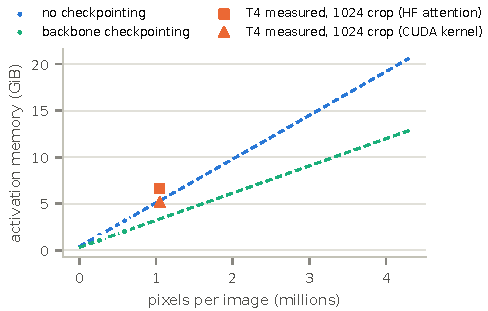
\includegraphics[width=0.62\textwidth]{figures/fig_memory.pdf}
\caption{The activation memory of the full Swin-S Mask2Former as a function of the number of pixels per
image, measured on a CPU at 512 and 768 pixels (dots, with linear fits) and on a T4 at 1024 pixels.
Recomputing the backbone's activations during the backward pass (checkpointing) saves about a third.
\generatedby{book/make\_book\_figures.py:fig\_memory}}
\label{fig:train-memory}
\end{figure}

\section{Faster kernels, proven identical *}\label{sec:train-kernels}
Three engineering changes made each training step faster. We required that no change to the speed may
change the mathematics, and we checked each change against the reference implementation before any
money was spent.

\subsection{A CUDA kernel for deformable attention}\label{sec:train-cuda}
Hugging Face computes the deformable attention of the pixel decoder (Equation~\eqref{eq:tr-deform}) with
a Python loop around \texttt{grid\_sample}. The same library ships a compiled CUDA kernel for the same
operation as part of its Deformable DETR model. We switched this kernel in, and compared it with the
reference on the shapes used in training, using random inputs whose sampling points extended slightly
beyond the edges of the feature maps. The outputs, and most of the gradients, agreed to within about
$10^{-5}$ in relative terms. The gradient with respect to the sampling \emph{locations} did not: at
2048 pixels its largest error was 1.2\%.

The cause turned out to be a property of bilinear interpolation (Figure~\ref{fig:train-kink}). A
bilinear sample is a continuous function of its location, but its derivative with respect to the
location jumps at every pixel centre. A point that lies within a millionth of a pixel of a centre can
land on either side of it, depending on how float32 arithmetic rounds its coordinates, and its gradient
then takes one value or the other. The test that settled the question computed a reference in float64,
and measured, for every large error, how far the point lay from the nearest crossing of a pixel centre.
Every large error lay within $7\times10^{-6}$ pixels of such a crossing, and the reference's \emph{own}
float32 loop showed the same errors in the same places. Away from the crossings, the kernel agreed with
the reference to $7\times10^{-6}$. Listing~\ref{lst:train-kernel} shows the essential part of the test.

\begin{figure}[t]
\centering
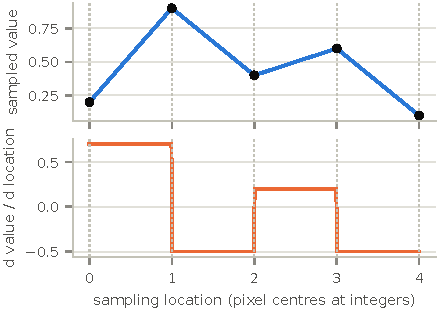
\includegraphics[width=0.62\textwidth]{figures/fig_kink.pdf}
\caption{Bilinear sampling along one axis. The sampled value (top) is continuous in the sampling
location, but its derivative (bottom) jumps at every pixel centre, so a gradient evaluated at a point
very close to a centre depends on which side of the centre rounding places the point.
\generatedby{book/make\_book\_figures.py:fig\_kink}}
\label{fig:train-kink}
\end{figure}

\begin{lstlisting}[caption={The kernel check: a float64 reference, and large errors allowed only at
kinks. Condensed from \file{experiments/exp\_139\_mask2former/src/fast\_ops.py}.},label=lst:train-kernel]
for name, function, dtype in (("truth", REFERENCE_MSDA, torch.float64),
                              ("kernel", kernel, torch.float64),
                              ("hf_float32", REFERENCE_MSDA, torch.float32)):
    inputs = [t.detach().to(device=device, dtype=dtype).clone().requires_grad_(True)
              for t in (value, locations, weights)]
    output = function(inputs[0], shapes, inputs[1], inputs[2])
    output.backward(grad_output.to(device=device, dtype=output.dtype))
    results[name] = [output.detach().double()] + [t.grad.double() for t in inputs]
# distance of every sampling point from the nearest pixel-centre crossing, per level
x = grid[..., 0] * widths - 0.5
y = grid[..., 1] * heights - 0.5
distance = torch.minimum((x - x.round()).abs(), (y - y.round()).abs())
near = distance < 1e-3                  # errors here are rounding at a kink, not a bug
passed = (errors["output"] <= 1e-4 and errors["grad_value"] <= 1e-4
          and errors["grad_weights"] <= 1e-4
          and errors["grad_locations_away_from_kinks"] <= 1e-4)
\end{lstlisting}

\subsection{Batched matching}\label{sec:train-matching}
The Hugging Face matcher copies one cost matrix from the GPU to the CPU for every image and for every
one of the ten predictions per step, which amounts to 80 stalls per step at a batch size of 8. Our
replacement computes all the matrices first, copies them once, and solves them on the CPU. We proved it
identical to the reference, bit for bit, on the loss and on all 161 gradient tensors of a small test
model, including the random draws of sampling points, which were made in the reference's order. On a
T4 it saved no measurable time, and we kept it only because it was proven harmless.

\subsection{A faster data loader}\label{sec:train-loader}
Our final loader decodes the photographs once into shared memory before the loader's worker processes
start. It decodes each annotated mask once and keeps only the crop of its bounding box, and it applies
the brightness augmentation and the normalisation on the GPU, starting from 8-bit pixels. A key-by-key
comparison with the first loader found no differences in the masks, and differences in pixel values
below $10^{-6}$, caused by float32 rounding in the gamma curve. The CPU time per sample fell from 80 to
19 milliseconds.

\subsection{How much faster?}\label{sec:train-speed}
The kernel reduced the time of a T4 step on two crops from 1.43 to 1.16 seconds, a speed-up of 1.24.
Profiling also corrected a guess that we had made beforehand. We had expected a speed-up of 1.5 to 2.5
times, but deformable attention accounted for only about a quarter of a step, so no kernel for it could
have delivered that.

\section{Exact gradient accumulation *}\label{sec:train-accumulation}
The final run used a batch of 8 in a single forward pass on a GPU with 80 GB or more of memory.
Cheaper cards with 24 GB could hold only two crops at a time, and the standard remedy for this,
\keyterm{gradient accumulation}, turned out to be subtly wrong for this loss.

Gradient accumulation splits a batch into $P$ micro-batches, runs the forward and backward passes on
each, and sums the gradients before taking a single optimiser step. The usual recipe divides the loss of
each micro-batch by $P$. This reproduces the full batch only if the loss of each micro-batch is an
average over parts of equal size, and the loss of Mask2Former is not. Its mask and Dice terms are
divided by the number of annotated masks \emph{in the current forward pass}, $n_b$, and its class term
by the total class weight in that pass, $w_b$, which counts one for each matched query and 0.1 for
each unmatched one. The loss of the whole batch is
\begin{equation}
\mathcal{L} = \frac{1}{N}\sum_b S^{\text{mask}}_b + \frac{1}{W}\sum_b S^{\text{cls}}_b,
\qquad N = \sum_b n_b,\quad W = \sum_b w_b,
\end{equation}
where $S^{\text{mask}}_b$ and $S^{\text{cls}}_b$ are the unnormalised sums of micro-batch $b$. Each
micro-batch reports the losses $\mathcal{L}^{\text{mask}}_b = S^{\text{mask}}_b/n_b$ and
$\mathcal{L}^{\text{cls}}_b = S^{\text{cls}}_b/w_b$, so the exact recombination weights each of them by
its \emph{share} of the batch:
\begin{equation}
\mathcal{L} = \sum_b \Big(\frac{n_b}{N}\,\mathcal{L}^{\text{mask}}_b + \frac{w_b}{W}\,\mathcal{L}^{\text{cls}}_b\Big).
\label{eq:train-shares}
\end{equation}
Dividing by $P$ instead would give a micro-batch containing one filament as much weight as one
containing twenty. Listing~\ref{lst:train-shares} implements Equation~\eqref{eq:train-shares}.

\begin{lstlisting}[caption={Scaling each micro-batch by its exact share. Condensed from
\file{experiments/exp\_139\_mask2former/src/train.py}.},label=lst:train-shares]
def step_shares(classes, num_queries, eos):
    masks = sum(len(item) for item in classes)                          # n_b
    weight = sum(len(item) + eos * (num_queries - len(item)) for item in classes)   # w_b
    return float(masks), float(weight)

def step_losses(model, pending, captured):
    counts = [step_shares(classes, 100, 0.1) for _, _, classes in pending]
    total_masks = sum(c[0] for c in counts)                            # N
    total_weight = sum(c[1] for c in counts)                           # W
    for (pixels, masks, classes), (n_b, w_b) in zip(pending, counts):
        model(pixel_values=pixels, mask_labels=masks, class_labels=classes)
        loss = sum(term * (w_b / total_weight if "cross_entropy" in key else n_b / total_masks)
                   for key, term in captured["dict"].items())          # the exact shares
        loss.backward()                                                # gradients accumulate
\end{lstlisting}

We tested the two recipes on a CPU with a small model, deterministic point sampling, and four samples
containing 6, 5, 1 and 1 filaments, split into two micro-batches, and measured the difference from a
single full batch:
\begin{center}\small
\begin{tabular}{@{}lcc@{}}
\toprule
accumulation & difference in loss & difference in gradient norm \\
\midrule
exact shares (Equation~\ref{eq:train-shares}) & $9.8\times10^{-8}$ & $1.4\times10^{-6}$ \\
division by the number of parts & $1.5\times10^{-3}$ & $4.1\times10^{-1}$ \\
\bottomrule
\end{tabular}
\end{center}
With exact shares, a card with 24 GB can train the same model that a larger card trains, at a fraction
of the price. This is what makes a cheaper run on the full data possible (Section~\ref{sec:sub-next}).

\section{The training run}\label{sec:train-run}
We trained the model on a rented H100 NVL GPU with 94 GB of memory, at \$2.59 an hour, with a spending
cap of \$6.50. The first attempt failed 53 seconds after training began. The machine's image set an
environment variable that asked the Hugging Face downloader to use an accelerator package which the
image did not contain. Our free rehearsals on Kaggle could not have caught this, because Kaggle does not
set that variable. Every check before that point had passed on the rented machine itself, including the
check that our scorer reproduces a known validation score to every printed digit. The fix was a single
environment variable, and the failed attempt cost about ten cents.

The second attempt ran all 50 epochs: 12,150 steps with a batch of 8, each in a single forward pass,
with no gradient accumulation and no activation checkpointing. Before its first step it checked the
CUDA kernel against the reference on the H100. After 45 steps it measured 0.464 seconds per step,
projected a total cost of \$5.25 including a reserve, and committed to all 50 epochs. It held 0.47
seconds per step and 39.35 GiB of memory throughout, and every five epochs it scored the validation
split (Figure~\ref{fig:train-curve}):
\begin{center}\footnotesize
\setlength{\tabcolsep}{3.5pt}
\begin{tabular}{@{}lcccccccccc@{}}
\toprule
epoch & 5 & 10 & 15 & 20 & 25 & 30 & 35 & 40 & 45 & 50 \\
\midrule
validation PQ & 0.420 & 0.420 & 0.441 & 0.444 & 0.440 & 0.457 & 0.460 & \textbf{0.468} & 0.467 & 0.464 \\
\bottomrule
\end{tabular}
\end{center}

\begin{figure}[t]
\centering
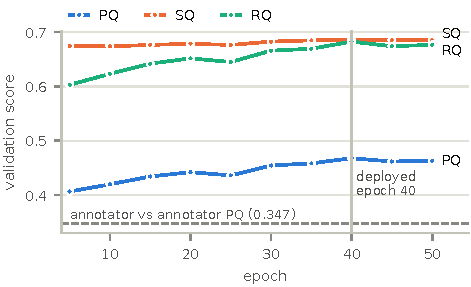
\includegraphics[width=0.7\textwidth]{figures/fig_curve.pdf}
\caption{Validation PQ, SQ and RQ of the final run, scored every five epochs during training, with
inference in bfloat16. PQ peaks at epoch 40, and the gains and losses late in training are mostly in
recognition. \generatedby{paper/make\_figures.py}}
\label{fig:train-curve}
\end{figure}

Two features of this curve deserve comment. First, the model improved until epoch 40, and then declined
slightly as the learning rate approached zero: at epoch 50 it found fewer filaments (813 true positives
against 872) and made fewer false detections. Second, epoch 40 was \emph{chosen} on the same validation
split on which it is scored. The best of ten candidates is optimistic by some amount, so the reported
score of 0.4705 includes the effect of this selection. The leaderboard, which played no part in the
selection, showed 0.41 for epoch 40 and 0.40 for epoch 50.

The whole run, including the failed first attempt, cost about \$4.80. The weights, 275,763,231 bytes per
checkpoint, were uploaded to a private Kaggle dataset, and we checked the dataset's listing before
deleting the rented machine.

A later run (exp142), intended to train on all 1,154 records, stopped within minutes on three rented
machines in a row. Our first diagnosis, which we wrote into the log, was that the account had run out of
credit. It was wrong. The diagnostics that the run itself had uploaded showed a
\texttt{ZeroDivisionError}: the projection of the budget divided by the interval between evaluations,
which a run on the full data sets to zero, and the machine's error handler had then stopped the machine,
as it was designed to do. The diagnostics that a failed run leaves behind should be read before the
infrastructure is blamed.

\section*{Exercises}
\begin{exercise}{Grid ceilings}
Reproduce the table of Section~\ref{sec:train-resolution} for cells of 2, 4 and 8 pixels on 200
training annotations: average each mask onto the coarse grid, enlarge it bilinearly, threshold it at
one half, and compute its IoU with the original. Then repeat the calculation with a binary encoding, in
which a cell is on if it is more than half covered, and compare the results.
\end{exercise}

\begin{exercise}{Steps per epoch}
With 974 records, two crops per record per epoch, and eight crops (or their equivalent) per step, how
many optimiser steps does an epoch have, and how many of them use whole frames? How many whole-frame
steps does the full run take?
\end{exercise}

\begin{exercise}{Clipping and Adam}
Show that if every gradient is multiplied by the same constant $c>0$, the update of
Equation~\eqref{eq:train-adamw} does not change, if we ignore $\epsilon$ and the weight decay. Then
explain what clipping every step to a fixed norm \emph{does} change.
\end{exercise}

\begin{exercise}{Accumulation by shares}
Two micro-batches contain 1 and 11 annotated masks, and their mask losses are 0.9 and 0.3. What is the
mask loss of the full batch, and what does dividing by the number of parts give instead?
\end{exercise}

\begin{exercise}{The kink}
Write bilinear interpolation along one axis, and its derivative with respect to the sampling location.
Evaluate the derivative in float32 at points $10^{-7}$ pixels on either side of a pixel centre, and
show that the two values differ by the difference between the neighbouring slopes.
\end{exercise}
